\documentclass[a4paper,14pt]{extarticle}

\usepackage[utf8x]{inputenc}
\usepackage[T1,T2A]{fontenc}
\usepackage[russian]{babel}
\usepackage{hyperref}
\usepackage{indentfirst}
\usepackage{here}
\usepackage{array}
\usepackage{graphicx}
\usepackage{caption}
\usepackage{subcaption}
\usepackage{chngcntr}
\usepackage{amsmath}
\usepackage{amssymb}
\usepackage{amsthm}
\usepackage{pgfplots}
\usepackage{pgfplotstable}
\usepackage[left=2cm,right=2cm,top=2cm,bottom=2cm,bindingoffset=0cm]{geometry}
\usepackage{multicol}
\usepackage{askmaps}
\usepackage{titlesec}
\usepackage{listings}
\usepackage{color}
\usepackage{enumerate}
\usepackage{hhline}
\usepackage{enumitem}
\usepackage{courier}
\usepackage{wrapfig}
\usetikzlibrary{arrows,automata}

\setitemize{itemsep=0em}
\setenumerate{itemsep=0em}

\theoremstyle{definition}

\pgfkeys{/pgf/number format/.cd,1000 sep={\,}}

\definecolor{green}{rgb}{0,0.6,0}
\definecolor{gray}{rgb}{0.5,0.5,0.5}
\definecolor{purple}{rgb}{0.58,0,0.82}

\lstset{
	language=python,
	backgroundcolor=\color{white},   
	commentstyle=\color{green},
	keywordstyle=\color{blue},
	numberstyle=\tiny\color{gray},
	stringstyle=\color{purple},
	basicstyle=\footnotesize\ttfamily,
	breakatwhitespace=false,
	breaklines=true,
	captionpos=b,
	keepspaces=true,
	numbers=left,
	numbersep=5pt,
	showspaces=false,
	showstringspaces=false,
	showtabs=false,
	tabsize=2,
	frame=single,
	inputpath={../code/}
}

\renewcommand{\le}{\ensuremath{\leqslant}}
\renewcommand{\leq}{\ensuremath{\leqslant}}
\renewcommand{\ge}{\ensuremath{\geqslant}}
\renewcommand{\geq}{\ensuremath{\geqslant}}
\renewcommand{\epsilon}{\ensuremath{\varepsilon}}
\renewcommand{\phi}{\ensuremath{\varphi}}
\renewcommand{\thefigure}{\arabic{figure}} 	
\newcommand{\norm}[1]{\left\lVert#1\right\rVert}
\newcommand*\sfrac[2]{{}^{#1}\!/_{#2}}

%\titleformat*{\section}{\large\bfseries} 
\titleformat*{\subsection}{\normalsize\bfseries} 
\titleformat*{\subsubsection}{\normalsize\bfseries} 
\titleformat*{\paragraph}{\normalsize\bfseries} 
\titleformat*{\subparagraph}{\normalsize\bfseries} 

\counterwithin{figure}{section}
\counterwithin{equation}{section}
\counterwithin{table}{section}
\newcommand{\sign}[1][5cm]{\makebox[#1]{\hrulefill}}
\graphicspath{{../pics/}}
\captionsetup{justification=centering,margin=1cm}
\setlength\parindent{5ex}
\def\arraystretch{1.3}
\def\tabcolsep{12pt}
%\titlelabel{\thetitle.\quad}

\DeclareMathOperator*{\argmin}{argmin}
\DeclareMathOperator*{\argmax}{argmax}

\begin{document}

\begin{titlepage}
\begin{center}
	\textbf{Санкт-Петербургский Политехнический Университет \\Петра Великого}\\[0.3cm]
	\small Институт компьютерных наук и технологий \\[0.3cm]
	\small Кафедра компьютерных систем и программных технологий\\[4cm]
	
	\textbf{ОТЧЕТ}\\ \textbf{по расчетному заданию}\\[0.5cm]
	\textbf{<<Построение моделей>>}\\[0.1cm]
	\textbf{Системный анализ и принятие решений}\\[8.0cm]
\end{center}

\begin{flushright}
	\begin{minipage}{0.4\textwidth}
		\begin{flushleft}
			\small \textbf{Работу выполнил студент}\\[3mm]
			\small группа 33501/4 \hspace*{6mm} Дьячков В.В.\\[5mm]
			
			\small \textbf{Преподаватель}\\[5mm]
		 	\small \sign[3cm] \hspace*{5mm} Сабонис С.С.\\[0.5cm]
		\end{flushleft}
	\end{minipage}
\end{flushright}

\vfill

\begin{center}
	\small Санкт-Петербург\\
	\small \the\year
\end{center}
\end{titlepage}

\addtocounter{page}{1}

\section{Техническое задание}

\begin{enumerate}
	\setlength{\itemsep}{0em}
	\item Привести задачу к канонической форме;
	\item Решить задачу геометрическим методом;
	\item Обозначить все опорные точки (в том числе недопустимые) и записать соответствующие им наборы базисных переменных, рассчитать значение целевой функции в каждой опорной точке (решить задачу методом полного перебора опорных точек);
	\item Решить задачу симплекс-методом в матричной форме;
	\item Решить задачу симплекс-методом в табличной форме;
	\item Ввести дополнительное ограничение, отсекающее оптимальную точку. Решить новую задачу двойственным симплекс-методом в табличной форме, в качестве начального базиса новой задачи использовать оптимальный базис исходной задачи;
	\item Сформулировать задачу, двойственную по отношению к исходной. 
\end{enumerate}

\section{Исходные данные}

\paragraph{Вариант 32}

Дана задача линейного программирования:
\begin{equation}
\label{eq:main}
\begin{cases}
	\max \left( 2 x_1 + 3 x_2 \right) \\
	x_1 + x_2 \le 4.8 \\
	-3 x_1 - x_2 \le -3.5 \\
	x_1 \ge 0 \\
	x_2 \ge 0
\end{cases}
\end{equation}

\section{Приведение к канонической форме}

Приведём задачу к канонической форме при помощи введения новых переменных:

\begin{equation}
\begin{cases}
	\max \left( 2 x_1 + 3 x_2 \right) \\
	x_1 + x_2 + x_3 = 4.8 \\
	-3 x_1 - x_2 + x_4 = -3.5 \\
	x_i \ge 0, i = \overline{1,4}
\end{cases}
\end{equation}
$x_1$ и $x_2$ -- свободные переменные, $x_3$ и $x_4$ -- базисные переменные. 

\section{Решение геометрическим методом}

На рис. \ref{pic:geometric_solution} изображено графическое представление системы \ref{eq:main}.

\begin{figure}[H]
\begin{center}
	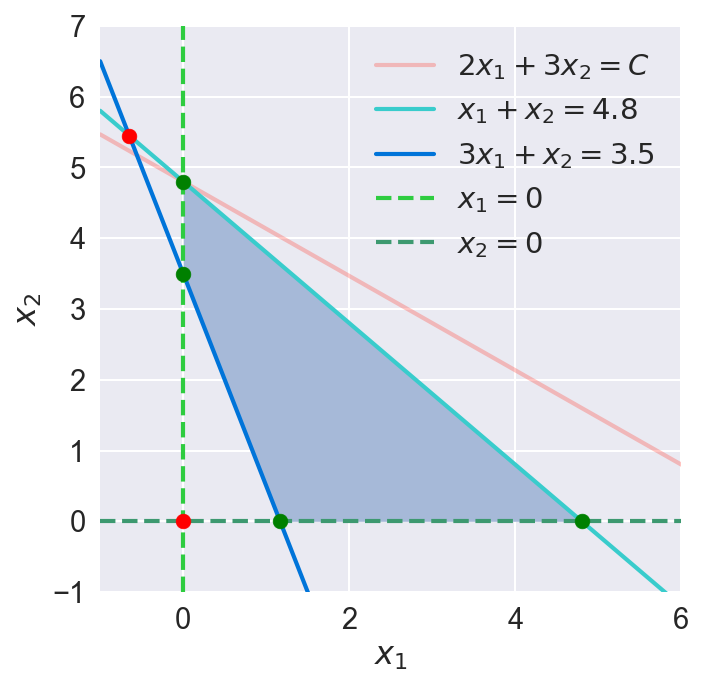
\includegraphics[scale=1]{system}
	\caption{Решение геометрическим методом}
	\label{pic:geometric_solution}
\end{center}
\end{figure}

Полученный выпуклый 4-угольник является областью допустимых решений. Зелеными точками на рисунке изображены допустимые опорные точки, красными -- недопустимые. Можно заметить, что максимальное значение в области допустимых значений прямая $2x_1 + 3x_2 = C$ принимает в точке $(0,\ 4.8)$, следовательно опорная точка $x_1 = 0$, $x_2 = 4.8$ является единственным решением задачи.

\section{Нахождение опорных точек}
\begin{equation}
\begin{cases}
	x_1 - x_2 = 1.6
	\\
	x_2 = 0
\end{cases}
\Rightarrow
\begin{cases}
	x_1 = 1.6
	\\
	x_2 = 0
\end{cases}
\end{equation}
\section{Решение симплекс-методом в матричной форме}

\section{Решение симплекс-методом в табличной форме}

\section{Введение дополнительного ограничения}

\section{Двойственная задача}

\end{document}